\section{Lasso}
    \subsection{超参数$\lambda$选择}
    调用R语言glmnet包,实现Lasso Regression,将数据分成十份,计算不同超参数$\lambda$下交叉验证(Cross Validation)的误差,并选择最优的超参数,结果如下图所示
    \begin{figure}[H]
        \centering
        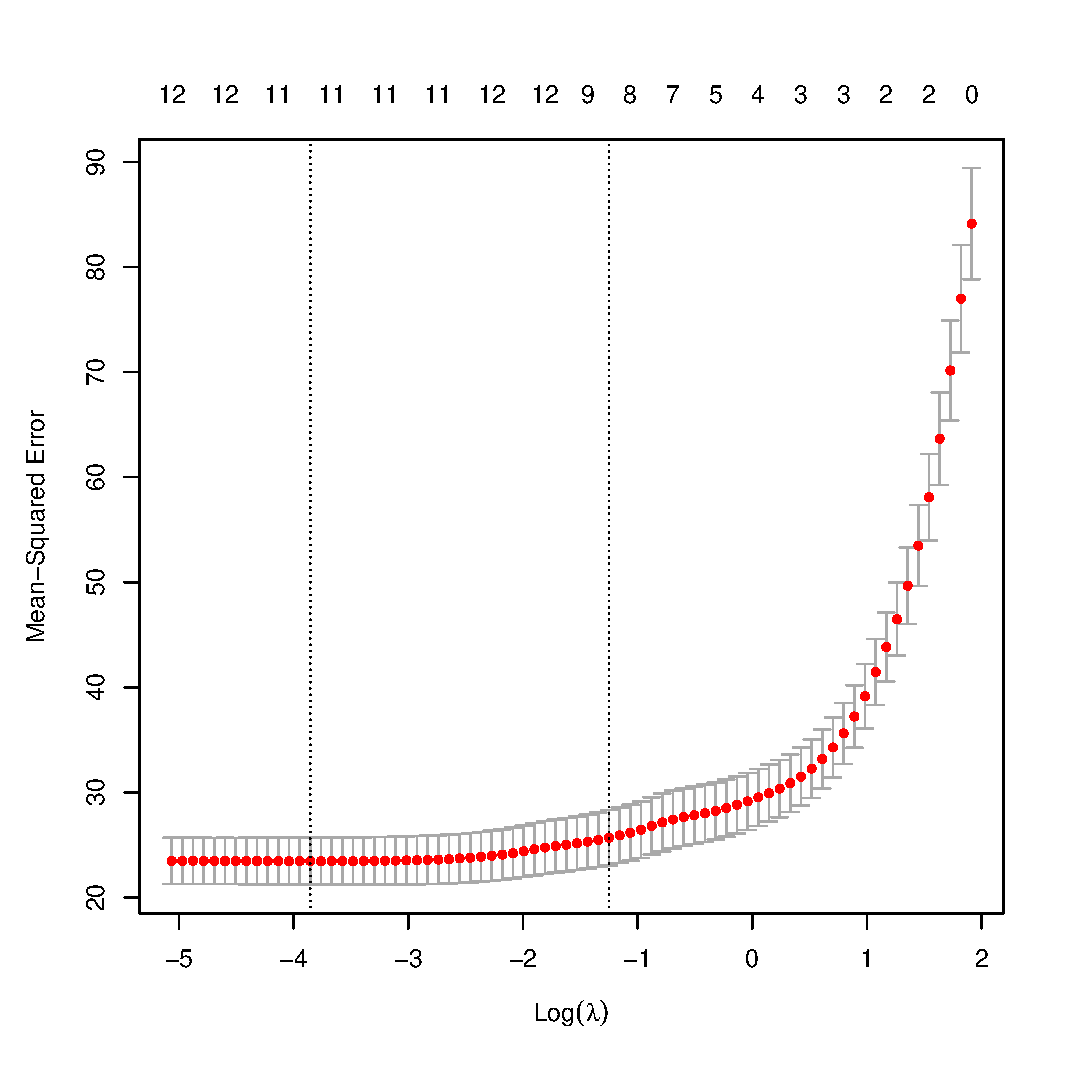
\includegraphics[width=0.6\textwidth]{lassocv.eps}
        \caption{Lasso Cross Validation}
    \end{figure}
    由结果可知,最优的$\lambda$取值约为0.021。
    \subsection{结果及分析}
    分别用glmnet包和自己编写的使用循环坐标下降法进行优化的代码在最优的$\lambda$取值下进行Lasso Regression,拟合得到的模型系数如下表所示
    \begin{table}[]
        \begin{tabular}{|c|c|c|c|c|c|c|c|c|c|c|c|c|c|c|}
        \hline
               & crim  & zn   & indus & chas & nox    & rm   & age  & dis   & rad  & tax   & ptratio & black & lstat & intercept \\ \hline
        glmnet & -0.10 & 0.04 & 0.00  & 2.69 & -16.57 & 3.85 & 0.00 & -1.42 & 0.26 & -0.01 & -0.93   & 0.01  & -0.52 & 34.91     \\ \hline
        ours   & -0.10 & 0.02 & -0.02 & 4.45 & -11.34 & 3.41 & 0.00 & -0.75 & 0.00 & 0.00  & 0.00    & 0.00  & -0.55 & 17.16     \\ \hline
        \end{tabular}
    \end{table}
    从表中我们可以看出,glmnet包的结果与我们的结果在各个项与房价的正负相关性上是相同的,但我们的结果将更多的系数压缩到0.
    
    在glmnet的结果中,房价与犯罪率、氮氧化物浓度、到就业中心的距离、学生与教师比例、人口数量呈负相关,与住宅用地比例、查尔斯河虚拟变量、每栋住宅的平均房间数、可达公路数、黑人比例呈正相关,与其余变量无关。

    在我们的结果中。房价与犯罪率、商场面积、氮氧化物浓度、到就业中心的距离、人口数量呈负相关,与住宅用地比例、查尔斯河虚拟变量、每栋住宅的平均房间数呈正相关,与其余变量无关。

    以上结果都与常识相符,接下来我们从MSE判断两种模型的优劣性,两种代码的MSE如下表所示
    \begin{table}[]
        \begin{tabular}{|c|c|}
        \hline
               & MSE   \\ \hline
        glmnet & 21.92 \\ \hline
        ours   & 27.72 \\ \hline
        \end{tabular}
    \end{table}
    有结果可见,glmnet包训练的模型MSE更小。
